
\graphicspath{{figures/modeling/gearTrain/}}
\section{Modeling of the Gear System}\label{sec:ModGearSys}
Three transfer functions are going to be determined in this section. First, the transfer of the motor's angular velocity $\omega_m$ to the angle of the arm $\theta_a$ through the gears. Then, two transfer functions are needed for $\tau_l$: the torque of the load comes from both the torque of the arm and stick $\tau_{as}$ and the frictions generated by the gears. Those transfer functions are shown in \autoref{fig:GearSystemDiagram}.
\begin{figure}[htbp]
	\centering
	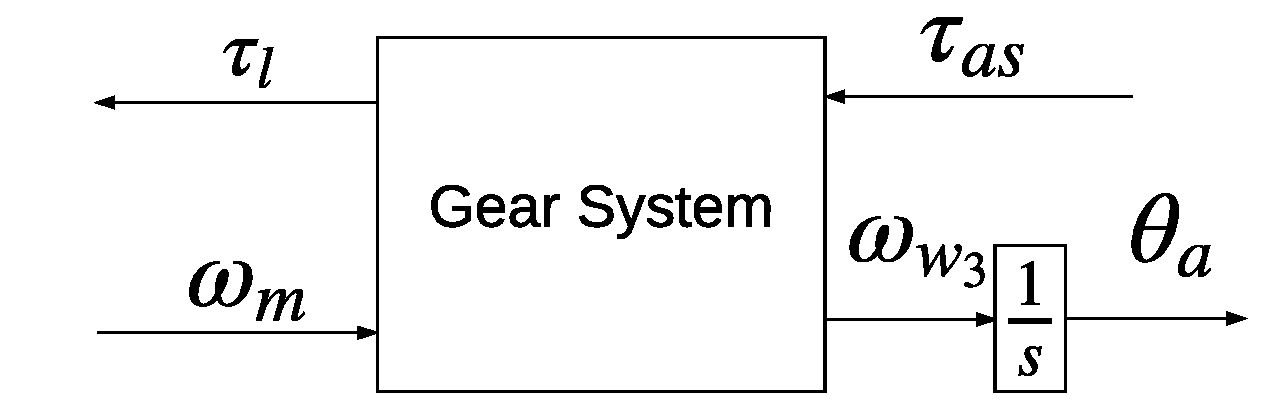
\includegraphics[width=0.6\textwidth]{GearSystemDiagram}
	\caption{Diagram of the angles and forces acting on the arm and the stick.}
	\label{fig:GearSystemDiagram}
\end{figure}

\startexplain
\explain{$\tau_l$ is the torque of the motor's load}{\si{\newton\meter}}
\explain{$\omega_m$ is the motor's angular velocity}{\si{\meter\per\second}}
\explain{$\tau_{as}$ is the torque of the arm and the stick}{\si{\newton\meter}}
\explain{$\omega_{w_3}$ is the third wheel's angular velocity}{\si{\meter\per\second}}
\stopexplain


\subsection{Relation between $\Omega_m$ and $\Theta_a$}

\begin{figure}[htbp]
	\centering
	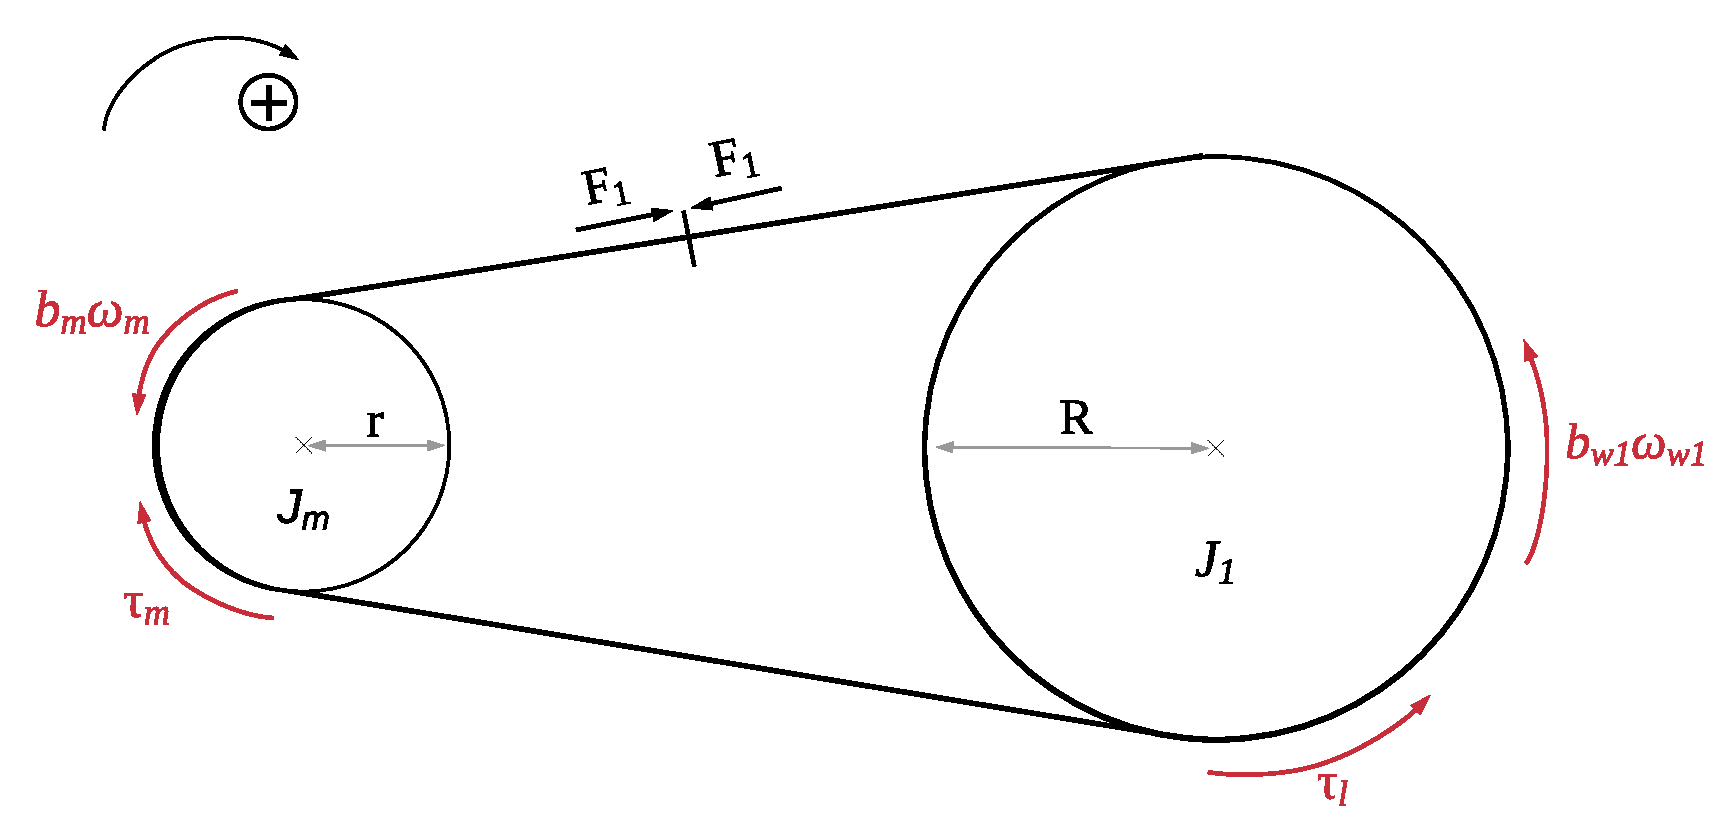
\includegraphics[width=0.9\textwidth]{figures/modeling/gearTrain/GearAndBeltSystem.pdf}
	\caption{Body diagram of the motor wheel system}
	\label{fig:Belt&Pulley}
\end{figure}

\startexplain
\explain{$J_m$ is the moment of inertia of the motor}{\si{\kilogram\meter\squared}}
\explain{$J_w$ is the moment of inertia of the wheel}{\si{\kilogram\meter\squared}}
\explain{$\omega_m$ is the motor's angular velocity}{\si{\meter\per\second}}
\explain{$\tau_m$ is the torque of the motor}{\si{\newton\meter}}
\explain{$F_1$ is the force transferred from the motor to the wheel}{\si{\newton}}
\explain{$r$ is the radius of the motor's wheel}{\si{\meter}}
\explain{$R$ is the radius of the wheel}{\si{\meter}}
\explain{$\tau_f$ is the torque of the gear train friction}{\si{\newton\meter}}
\explain{$\tau_L$ is the torque of the wheel's load}{\si{\newton\meter}}
\explain{$b_w$ is the viscous friction coefficient of the wheel}{\si{\newton\meter\second}}
\stopexplain


From \autoref{fig:Belt&Pulley}, considering the small wheel as the one connected to the motor, if the motor shaft turns, the belt joining the small and the big wheel will make them turn the same distance:
\begin{equation}
	\theta_m r = \theta_w R \addunit{\meter}
\end{equation}

This expression is then differentiated to find the relation with the angular velocities:
\begin{equation}
	\omega_m r = \omega_w R\addunit{\meter\per\second}
	\label{eq:AngularVelRelation}
\end{equation}

Then the gear ratio can be defined as: 
\begin{equation}
	N = \frac{r}{R} \addunit{1}
	\label{eq:GearRatio}
\end{equation}

As the gear system is composed by three similar connected wheels structures like shown in \autoref{fig:Belt&Pulley}, the ratio between small wheel x, $r_x$, and big wheel x, $R_x$ is the same:
\begin{equation}
	\frac{r_x}{R_x} = \frac{r_{motor}}{R_{w_1}} = \frac{r_{w_1}}{R_{w_2}} = \frac{r_{w_2}}{R_{w_3}} = N \addunit{1}
\end{equation}
Knowing this and since $\omega_m$ is transferred through three gears reductions, the relation between the angular velocity of the motor $\omega_m$ and the angle of the arm $\theta_a$ is found following the principle of \autoref{eq:AngularVelRelation}:
\begin{subequations} \label{eq:tech_ToA}
	\begin{flalign}
		&\omega_a(t) = N^3 \omega_m(t) \\
		&\theta_a(t) = N^3 \int_{0}^{t}\omega_m(v) dv \\
		&\mathcal{L}\{\theta_a(t)\} = \Theta_a(s) = N^3 \cdot \frac{1}{s} \Omega_m(s) \addunit{1}
	\end{flalign}
\end{subequations}

The transfer function from the motor's angle velocity to the angle of the arm is:
\begin{equation}\label{eq:thetaOmega}
	\frac{\Theta_a(s)}{\Omega_m(s)} =  \frac{N^3}{s} \addunit{1}
\end{equation}

\subsection{Finding $\tau_l$}

Now that the relationship between $\theta_a$ and $\omega_m$ is found, $\tau_l$ is studied. In the inverted pendulum case the load is composed of the friction and the torque necessary to counter the gravity and the momentums which result in \autoref{eq:TauL}.

\begin{equation}\label{eq:TauL}
	\tau_l = \tau_{gear} + \tau_{as} \addunit{\newton\meter}
\end{equation}
\startexplain
\explain{$\tau_{gear}$ is the load from the gear system}{\si{\newton\meter}}
\explain{$\tau_{as}$ is the load from the arm and the stick}{\si{\newton\meter}}
\stopexplain


\subsubsection*{Determining $\tau_{gear}$}
The gear train is composed by three identical belt and pulley system. \autoref{fig:Belt&Pulley} corresponds to the first system between the motor and the first wheel. 

Using the previously stated $2^{nd}$ law of motion, the mechanical equation for the motor wheel can be found from \autoref{fig:MotorBodyDiagram}:

\begin{equation}
    J_m \dot{\omega}_m = \tau_m + F_1r - b_m\omega_m \addunit{\newton\meter}
    \label{eq:MotorfreeBody}
\end{equation}

For the body diagram for the wheel in \autoref{fig:Belt&Pulley}:
\begin{equation}
	J_w\dot{\omega}_{w} = -F_1R -\tau_L -b_{w}\omega_{w} \addunit{\newton\meter}
\end{equation}

Looking at the whole gear train, $\tau_{gear}$ represents the total friction and $\tau_L$ is the opposite of the torque transferred to the next wheel. Which gives for wheels 1, 2 and 3:

\begin{subequations} 
	\begin{flalign} \label{eq:GiveMeAnOriginalName}
		&J_{w_1}\dot{\omega}_{w_1} = -F_1R + F_2r -b_{w_1}\omega_{w_1} \addunit{\newton\meter}\\ 
		&J_{w_2}\dot{\omega}_{w_2} = -F_2R + F_3r -b_{w_2}\omega_{w_2} \addunit{\newton\meter}\\ 
		&J_{w_3}\dot{\omega}_{w_3} = -F_3R - b_{w_3}\omega_{w_3} \addunit{\newton\meter}
	\end{flalign}
\end{subequations}

Using the relation in \autoref{eq:AngularVelRelation}, the angular velocity of each wheels can be found according to $\omega_m$:
\begin{subequations} 
	\begin{flalign}
		&\omega_{w_1} = N \omega_m \addunit{\radian\per\second}\\
		&\omega_{w_2} = N \omega_{w_1} = N^2 \omega_m \addunit{\radian\per\second}\\
		&\omega_{w_3} = N \omega_{w_2} = N^3 \omega_m \addunit{\radian\per\second}
	\end{flalign}
\end{subequations}

The same equations are valid with angular accelerations.
Which gives for Equations \ref{eq:GiveMeAnOriginalName}:
\begin{subequations} 
	\begin{flalign}  
		&J_{w_1}N\dot{\omega}_m = -F_1R + F_2r -b_{w_1}N\omega_m \addunit{\newton\meter}\\ 
		&J_{w_2}N^2\dot{\omega}_m = -F_2R + F_3r -b_{w_2}N^2\omega_m  \addunit{\newton\meter}\\ 
		&J_{w_3}N^3\dot{\omega}_m = -F_3R - b_{w_3}N^3\omega_m  \addunit{\newton\meter}
	\end{flalign}
\end{subequations}

In order to simplify the frictions, they are considered to be wet friction as such the frictions in the gear system are directly dependent on the angular velocity of the wheels. When the system is not moving:
\begin{subequations} 
	\begin{flalign}  \label{eq:TaufTgearConditions}
	\tau_L &= \tau_{gear}\\
	\omega_m &= 0
	\end{flalign}
\end{subequations}

Inserting \autoref{eq:TaufTgearConditions} into \autoref{eq:MotorfreeBody}:

\begin{equation} 
		\tau_{gear} = -F_1 \cdot r \addunit{\newton\meter}
		\label{eq:TaufF1r}
\end{equation}

$F_1$ needs to be isolated from \autoref{eq:GiveMeAnOriginalName}. Each forces $F_1$, $F_2$ and $F_3$ are then isolated, giving: 

\begin{subequations} 
	\begin{flalign}
		&F_1 = -\frac{1}{R} (b_{w_1}N\omega_m + J_{w_1}N\dot{\omega}_m - F_2r) \addunit{\newton} 	\label{eq:F1}\\ 
		&F_2 = -\frac{1}{R} (b_{w_2}N^2\omega_m +  J_{w_2}N^2\dot{\omega}_m - F_3r) \addunit{\newton}	\label{eq:F2}\\
		&F_3 = -\frac{1}{R} (b_{w_3}N^3\omega_m + J_{w_3}N^3\dot{\omega}_m)	\addunit{\newton}		\label{eq:F3}
	\end{flalign}
\end{subequations}

Inserting \autoref{eq:F3} in \autoref{eq:F2}, then \autoref{eq:F2} in \autoref{eq:F1}, the expression of $F_1$ according to the friction and moment of inertia of each wheel is found:

\begin{flalign}
	F_1 &=-\frac{1}{R} N(b_{w_1}\omega_m + J_{w_1}\dot{\omega}_m \notag \\
	& +\frac{r}{R} N^2(b_{w_2}\omega_m + J_{w_2}\dot{\omega}_m \notag \\
	& +\frac{r}{R} N^3(b_{w_3}\omega_m + J_{w_3}\dot{\omega}_m))) \addunit{\newton}
\end{flalign}


Using \autoref{eq:TaufF1r} and the gear ratio in \autoref{eq:GearRatio}, the total friction is given by: 
\begin{align} \label{eq:TaufTimeDomain}
	\tau_{gear} &= N^2 (b_{w_1}\omega_m + J_{w_1}\dot{\omega}_m \notag \\
	& +N^3 (b_{w_2}\omega_m + J_{w_2}\dot{\omega}_m \notag \\
	& +N^4 (b_{w_3}\omega_m + J_{w_3}\dot{\omega}_m))) \addunit{\newton\meter}
\end{align}


\autoref{eq:TaufTimeDomain} is Laplace-transformed:

\begin{flalign} \label{eq:TaufLaplaceDomain}
	\mathcal{L}\{\tau_{gear}(t)\} = \tau_{gear}(s) &= N^2 (B_{w_1}\Omega_m + sJ_{w_1}\Omega_m \notag \\
	& +N^3 (B_{w_2}\Omega_m + sJ_{w_2}\Omega_m \notag \\
	& +N^4 (B_{w_3}\Omega_m + sJ_{w_3}\Omega_m))) \addunit{1}
\end{flalign}


\autoref{eq:TaufLaplaceDomain} is reorganized to find the final expression for $\tau_{gear}$ in \autoref{eq:TaufReorganized}:
\begin{equation}
	\tau_{gear} = \left[(N^2 J_1 + N^5 J_2 + N^9 J_3)s +( N^2 B_1 + N^5 B_2 + N^9 B_3)\right]\Omega_m \addunit{1}
	\label{eq:TaufReorganized}
\end{equation}

The moments of inertia and the frictions of each parts of the gear train will be grouped into two variables, respectively $J_{gear}$ and $B_{gear}$:
\begin{equation}
	\tau_{gear} = (J_{gear}s +B_{gear})\Omega_m \addunit{1}
	\label{eq:TaufSimplified}
\end{equation}











\subsubsection*{Determining $\tau_{as}$}

$\tau_{as}$ is the torque necessary for the motor to counter the load applied by the arm and the stick. It can be divided into two parts as in \autoref{eq:TauasBegin}.

\begin{equation}\label{eq:TauasBegin}
	\tau_{as}=\tau_a+\tau_s \addunit{\newton\meter}
\end{equation}
\startexplain
\explain{$\tau_a$ is the load of the arm}{\si{\newton\meter}}
\explain{$\tau_s$ is the load of the stick}{\si{\newton\meter}}
\stopexplain

The first part is the torque to counter the load of the arm, $\tau_a$.
 
 \begin{figure}[htbp]
 	\centering
 	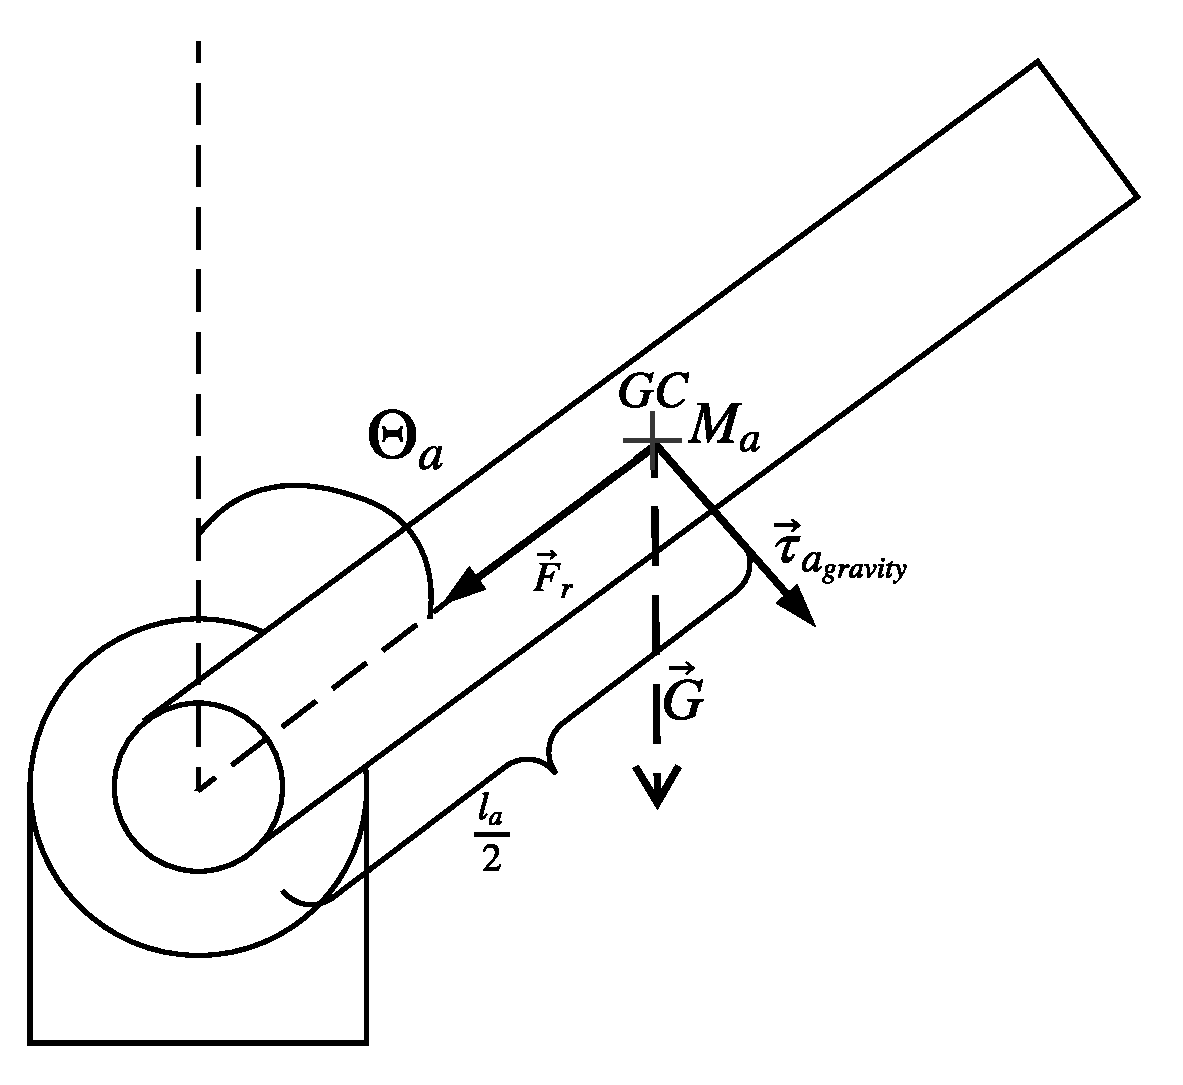
\includegraphics[width=0.5\textwidth]{PendulumWithWeightlessRod}
 	\caption{Approximation of the arm as a weightless rod pendulum}\label{fig:tauAgrav}
 \end{figure}
 \startexplain
 \explain{$\vec{G}$ is the gravity force}{\si{\kilogram\meter\per\second\squared}}
 \explain{$\vec{F}_r$ is the reaction force of the arm to the gravity}{\si{\kilogram\meter\per\second\squared}}
 \explain{$\tau_{a_{gravity}}$ is the torque remaining of the gravity after substracting $\vec{F}_r$}{\si{\newton\meter}}
 \explain{$l_a$ is the length of the arm}{\si{\meter}}
 \stopexplain
 
According to \autoref{fig:tauAgrav}, the $2^{nd}$ and the $3^{rd}$ Newton's law \autoref{eq:tauA} can be deduced.

\begin{equation}\label{eq:tauA}
	J_a \ddot{\theta}_a=\vec{G}_a-\tau_a \addunit{\newton\meter}
\end{equation}
\startexplain
\explain{$M_a$ is the mass of the arm}{\si{\kilogram}}
\explain{$\tau_a$ is the reaction torque from the motor}{\si{\newton\meter}}
\explain{$J_a$ is the moment of inertia of the arm}{\si{\kilogram\meter\squared}}
\stopexplain

By assuming the arm to be a pendulum with a weightless rod and by geometry law \autoref{eq:tauA} can be derived into \autoref{eq:tauARot}

\begin{equation}\label{eq:tauARot}
	\tau_a=-J_a\ddot{\theta}_a+\frac{l_a}{2}M_a g sin(\theta_a) \addunit{\newton\meter}
\end{equation}

By linearizing \autoref{eq:tauA}, \autoref{eq:finalTauA} is derived.

\begin{flalign}\label{eq:finalTauA}
	\tau_a&=-J_a \ddot{\theta}_a+M_a g \frac{l_a}{2} \theta_a \addunit{\newton\meter} \notag\\
	\mathcal{L}\{\tau_a\}=\tau_a(s)&=-J_a\Theta_a s^2+M_a g \frac{l_a}{2} \Theta_a \addunit{1}
\end{flalign}

Now, the load of the stick $\tau_s$ is studied. Unlike the arm, it is not directly connected to the gear train, so it  has to be defined in a new base in order to be used with the arm. The Fresnel base has $\tau_s$ is on one of the axis as seen in \autoref{fig:loadStick}.

 \begin{figure}[htbp]
 	\centering
 	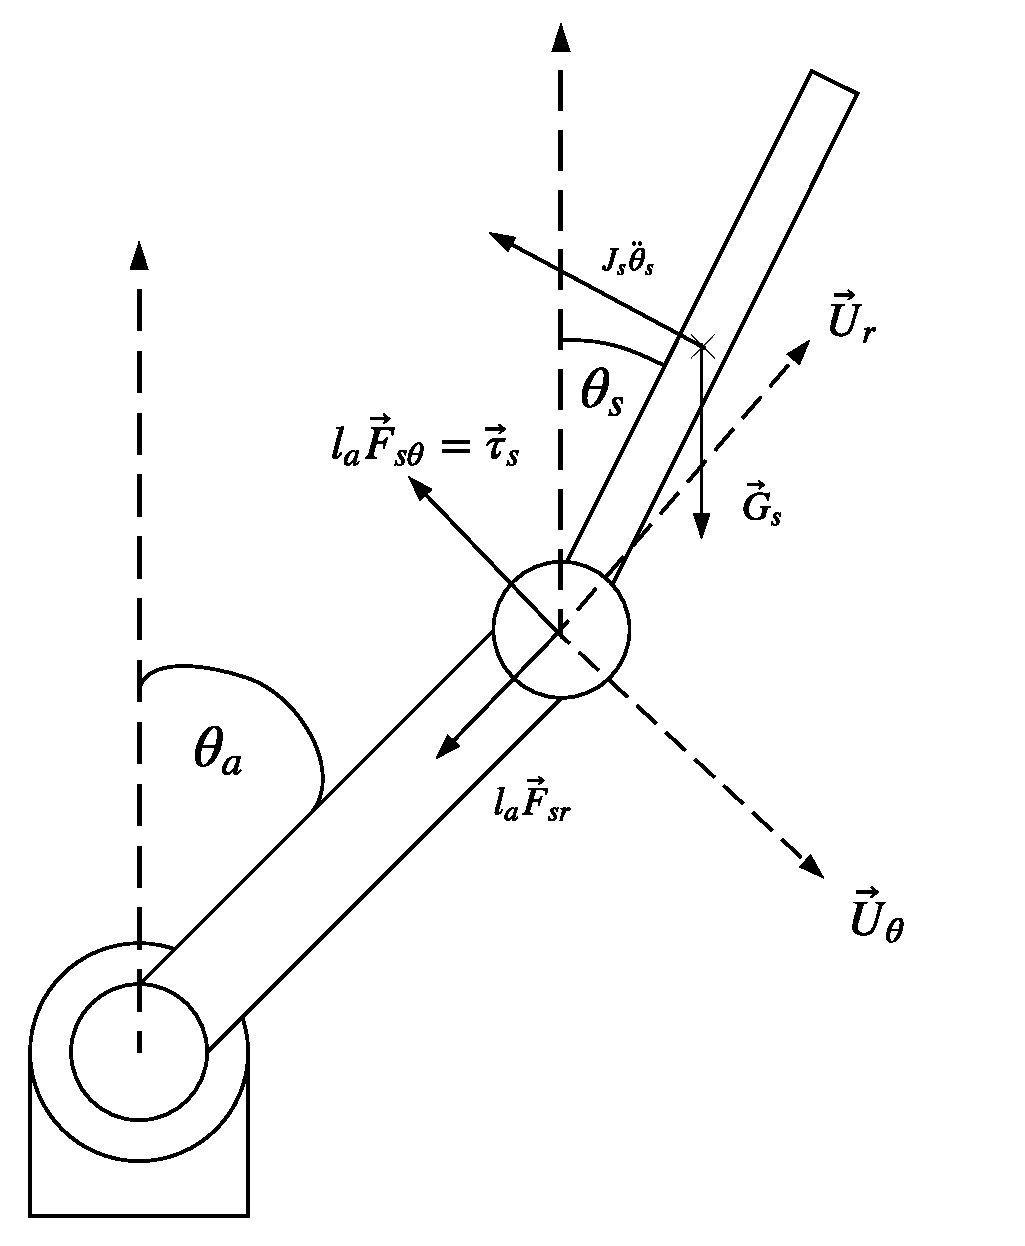
\includegraphics[width=0.5\textwidth]{loadOnThetaA}
 	\caption{Load applied by the stick translated in the Fresnel base}\label{fig:loadStick}
 \end{figure}
 \startexplain
 \explain{$\vec{G}_s$ is the gravity force applied on the stick}{\si{\kilogram\meter\per\second\squared}}
 \explain{$\vec{F}_{sr}$ is the reaction force of the arm to the load of the stick}{\si{\kilogram\meter\per\second\squared}}
 \explain{$\vec{F}_{s\theta}$ is the force generated by the stick}{\si{\kilogram\meter\per\second\squared}}
 \explain{$\tau_{s}$ is the load applied by the stick on the gear train}{\si{\newton\meter}}
 \explain{$l_a$ is the length of the arm}{\si{\meter}}
 \stopexplain

This gives, by Newton's $2^{nd}$ law, \autoref{eq:tauSBase}

\begin{subequations}\label{eq:tauSBase}
	\begin{flalign}
		J_s\vec{\ddot{\theta}}_{s\theta}&=\vec{G}_{s\theta}+\vec{F}_{s\theta} \addunit{\newton\meter}\\
		J_s\vec{\ddot{\theta}}_{sr}&=\vec{G}_{sr}+\vec{F}_{sr} \addunit{\newton\meter} \addunit{\newton\meter}
	\end{flalign}
\end{subequations}

As said in \autoref{fig:loadStick}, $\vec{F}_{sr}$ is the reaction force from the arm, and since it is assumed that the arm is incompressible, this force is cancelled. This leaves only a dependency on $\vec{U}_{\theta}$, which, by applying geometric properties, gives \autoref{eq:Fso}.

\begin{flalign}\label{eq:Fso}
	-cos(\theta_a-\theta_s)J_s\ddot{\theta}_s&=-M_sg\left(l_asin(\theta_a)+\frac{l_s}{2}sin(\theta_s)\right)cos(\theta_a) \notag\\
	&+l_aF_{s\theta} \addunit{\newton\meter}
\end{flalign}

\autoref{eq:Fso} combined with Newton $3^{rd}$ law gives $\tau_s$ as explained in \autoref{eq:tauS}.

\begin{subequations}\label{eq:tauS}
	\begin{flalign}
		\tau_s&=l_aF_{s\theta} \addunit{\newton\meter}\\
		\tau_s&=-cos(\theta_a-\theta_s)J_s\ddot{\theta}_s+M_sg\left(l_asin(\theta_a)+\frac{l_s}{2}sin(\theta_s)\right)cos(\theta_a)\addunit{\newton\meter}
	\end{flalign}
\end{subequations}

By linearizing \autoref{eq:tauS}, \autoref{eq:LinTauS} is found.

\begin{flalign}\label{eq:LinTauS}
	\tau_s = -J_s \ddot{\theta_s} s^2 + M_s g \left(\theta_a l_a+\frac{l_s}{2}\theta_s\right) \addunit{\newton\meter}    
\end{flalign}

When controlling the equilibrium of the stick, $\theta_s$ grows up to only a couple degrees, not exceeding 10. Therefore, regarding the torque generated by the stick, $\theta_s$ can be considered as 0. Thus giving:

\begin{equation}\label{eq:FinalTauS}
	\mathcal{L}\{\tau_{s}\}=\tau_{s}(s)=M_sgl_a\Theta_a \addunit{1}
\end{equation}



At last $\tau_{as}$ is found by combining Equations \eqref{eq:finalTauA} and \eqref{eq:FinalTauS} in \autoref{eq:FinalTauAS}.

\begin{subequations}\label{eq:FinalTauAS}
	\begin{flalign}
		\tau_{as} &=\tau_a+\tau_s \addunit{\newton\meter}\\
		&= -J_a\Theta_a s^2+M_a g \frac{l_a}{2} \Theta_a+M_sgl_a\Theta_a  \addunit{1}
	\end{flalign}
\end{subequations} 

By combining Equations \eqref{eq:TauL}, \eqref{eq:FinalTauAS} and \eqref{eq:TaufSimplified}, $\tau_l$ is then defined as \autoref{eq:finalTauL}.

\begin{equation}\label{eq:finalTauL}
	\tau_l=M_ag\frac{l_a}{2}\Theta_a-J_a\Theta_a s^2+M_sgl_a\Theta_a +(J_{gear}s +B_{gear})\Omega_m(s)
\end{equation}

Now that $\tau_l$ is found, it is re-injected in \autoref{eq:Iinserted} giving \autoref{eq:begTFOaUm}.

\begin{align}\label{eq:begTFOaUm}
s J_{m} \Omega_m(s) &=K_{t} \frac{U_m-K_e \Omega_m(s)}{R_m} - \Big(M_ag\frac{l_a}{2}\Theta_a-J_a\Theta_a s^2 +M_sgl_a\Theta_a \notag \\ 
&+ (J_{gear}s +B_{gear})\Omega_m(s)\Big) - B_{m} \Omega_m(s) 
\end{align}

$\Omega_m(s)$ is expressed according to $\Theta_a$ with \autoref{eq:thetaOmega}.

\begin{flalign}\label{eq:begTFOaUm2}
\frac{J_{m}}{N^3}\Theta_a s^2 &=K_{t} \frac{U_m-K_e \frac{s}{N^3}\Theta_a}{R_m}- \Big(M_ag\frac{l_a}{2}\Theta_a-J_a\Theta_as^2 +M_sgl_a\Theta_a   \notag \\ 
&+ (J_{gear}s +B_{gear})\frac{s}{N^3}\Theta_a\Big) - B_{m} \frac{s}{N^3}\Theta_a 
\end{flalign}


Factorizing \autoref{eq:begTFOaUm2} by $\Theta_a$ and $U_m$, \autoref{eq:midTFOaUm} is obtained.

\begin{flalign}\label{eq:midTFOaUm}
\frac{K_t}{R_m}U_m	&= \Theta_a\Big[ \frac{J_{m}}{N^3}s^2 + \frac{K_e K_t}{R_mN^3}s + M_ag\frac{l_a}{2} - J_a s^2 + M_sgl_a \notag \\
					&+ \frac{J_{gear}}{N^3}s^2+\frac{B_{gear}}{N^3}s + \frac{B_{m}}{N^3}s \Big]
\end{flalign}

\autoref{eq:midTFOaUm} is then organized to find $\nicefrac{\Theta_a}{U_m}$.
\begin{flalign}\label{eq:UmThetaaTFSimplified}
\frac{\Theta_a}{U_m}&= \frac{\nicefrac{K_t}{R_m}}{\left( \frac{J_{m}}{N^3} + \frac{J_{gear}}{N^3} - J_a \right)s^2 + \left( \nicefrac{1}{N^3}\left( \frac{K_e K_t}{R_m} + B_{gear} + B_{m}\right) \right) s + gl_a(M_s+M_a)}
\end{flalign}




%

Now that $\tau_l$ is found, it is re-injected in \autoref{eq:Iinserted} giving \autoref{eq:UmtoThetaa1}. 
\begin{flalign}\label{eq:UmtoThetaa1}
	s\cdot J_m\cdot \Omega_m(s) & =K_t\frac{U_m(s)-K_e\cdot \Omega_m(s)}{R_m+sL_m}-\big(-J_a\Theta_a s^2+M_ag\frac{l_a}{2}\Theta_a \notag \\ 
	& +M_sl_a\Theta_a+s^2\frac{l_s}{2}l_aM_s\Theta_a+s^2\frac{l_s^2}{4}M_s\left(\frac{\frac{-3l_a}{2l_s}s^2}{s^2-\frac{3g}{2l_s}}\right)\Theta_a \notag\\
	& +(J_{gear}s +B_{gear})\Omega_m(s) \big) - B_m \cdot \Omega_m(s)
\end{flalign}

$\Omega_m(s)$ is expressed according to $\Theta_a$ with \autoref{eq:thetaOmega}. 
\begin{flalign}\label{eq:UmtoThetaa2}
	s\cdot J_{m}\cdot \frac{s}{N^3}\Theta_a &=K_{t}\frac{U_m(s)-K_e\cdot \frac{s}{N^3}\Theta_a}{R_m+sL_m}-\Big( -J_a\Theta_a s^2+M_ag\frac{l_a}{2}\Theta_a \notag\\ 
	&+M_sl_a\Theta_a+s^2\frac{l_s}{2}l_aM_s\Theta_a+s^2\frac{l_s^2}{4}M_s\left(\frac{\frac{-3l_a}{2l_s}s^2}{s^2-\frac{3g}{2l_s}}\right)\Theta_a \notag \\
	&+(J_{gear}s+B_{gear}) \frac{s}{N^3}\Theta_a \Big)  - \frac{B_m}{N^3}s\Theta_a
\end{flalign}

\autoref{eq:UmtoThetaa2} is reorganized in order to find the transfer function from $U_m$ to $\Theta_a$. $L_m$ is neglected given the insignificance of it's value compared to $R_m$.
\begin{flalign}\label{eq:UmtoThetaa3}
	\frac{K_t}{R_m} U_m &= -\Theta_a \Big[s\cdot J_{m}\cdot \frac{s}{N^3} + \frac{K_eK_t}{R_m}-J_a s^2+M_ag\frac{l_a}{2} \notag\\ 
	&+M_sl_aa+s^2\frac{l_s}{2}l_aM_s+s^2\frac{l_s^2}{4}M_s\left(\frac{\frac{-3l_a}{2l_s}s^2}{s^2-\frac{3g}{2l_s}}\right) \notag \\
	&+(J_{gear}s+B_{gear}) \frac{s}{N^3} +\frac{B_{m}}{N^3}s \Big]
\end{flalign}

\begin{flalign}
	\frac{\Theta_a}{U_m} &= \frac{\frac{K_t}{R_m}(s^2-\frac{3g}{2l_s})}{As^4+Bs^3+Cs2+Ds+E} \label{eq:UmtoThetaaFinal}\\
	A&= \frac{J_m}{N^3} + \frac{J_{gears}}{N^3} - J_a + \frac{1}{8}l_al_sM_s \addunit{\kilo\gram\meter\squared}\\
	B&= \frac{1}{N^3}\left( \frac{K_eK_t}{R_m} + B_m + B_{gears} \right) \addunit{\newton\meter\second}\\
	C&= gl_a\left( M_a + \frac{1}{4}M_s \right) -\frac{3g}{2l_s}\left( \frac{J_m + J_{gears}}{N^3} -J_a\right) \addunit{\newton\meter}  \\
	D&= -\frac{3g}{2l_sN^3} \left( \frac{K_eK_t}{R_m} + B_m + B_{gears} \right) \addunit{\newton\meter\per\second}  \\
	E&= -\frac{3g^2l_a}{4l_s}(M_a+M_s)  \addunit{\newton\meter\per\second\squared}
\end{flalign}
%\subsubsection{Determining $\frac{\Theta_a}{U_m}$}


\todo[inline,author=Maxime]{Test to see the minimum torque to overcome dry friction}
As the motor torque combined with the gear is really large the load generated by the arm and the stick can be neglected. Indeed the motor has to use at least \SI{3.5}{\ampere} to move so it requires a torque of \SI{3.8}{\newton\meter} at the end of the gear train. On the other hand the torque load applied by the arm and stick without the momentum is around \SI{0.005}{\newton\meter} while the arm has to go at least 

Also due to their small value the inductance and the friction at joint of the arm and the stick are also neglected. Such assumptions means that the load on the motor comes then solely from the friction of the gears and the motor itself. This combined with Equations (\ref{eq:Iinserted}), (\ref{eq:TaufSimplified}) and (\ref{eq:thetaOmega}) gives \autoref{eq:begTFOaUm}.


\begin{align}\label{eq:begTFOaUm}
	s J_{m} \Omega_m(s) = &K_{t} \frac{U_m-K_e \Omega_m(s)}{R_m} \notag \\ 
	&- \Omega_m(s) (J_{gear}s+B_{gear}) - B_{m} \Omega_m(s) \addunit{1}
\end{align}

Factorizing \autoref{eq:begTFOaUm} by $\Omega_m$ and $U_m$ \autoref{eq:midTFOaUm} is obtained.

\begin{equation}\label{eq:midTFOaUm}
	\Omega_m(s)\left(s J_m+\frac{K_t K_e}{ R_m} + (J_{gear}s+B_{gear}) + B_{m}  \right)=\frac{U_m K_t}{R_m}	
\end{equation}

And so $\frac{\Omega_m}{U_m}$ i obtained in \autoref{eq:finTFOaUm}.
\begin{subequations}\label{eq:finTFOaUm}
	\begin{align}
		\Omega_m=&\Theta_a\frac{s}{N^3}\\
		\frac{\Omega_m(s)}{U_m}=&\frac{\frac{ K_t}{R_m}}{s(J_m+J_{gear})+\frac{K_t K_e +R_m (B_{gear}+B_m)}{R_m}} \\
		\frac{\Theta_a(s)}{U_m}=&\frac{N^3}{s}\frac{\frac{ K_t}{R_m}}{s(J_m+J_{gear})+\frac{K_t K_e +R_m (B_{gear}+B_m)}{R_m}}
	\end{align}
\end{subequations}

\newpage
Since it is a change in the small angles, the linearization of a cosine and a sine function gives \autoref{eq:BasLin}.

\begin{subequations}\label{eq:BasLin}
	\begin{flalign}
		&sin(x)=>x \addunit{1}\\
		&cos(x)=>1 \addunit{1}
	\end{flalign}
\end{subequations}

\autoref{fig:BasLinPlot} shows that, within an angle variation of \SI{10}{\degree}, the approximation of the linearization is acceptable.

\begin{figure}[htbp]
	\centering
	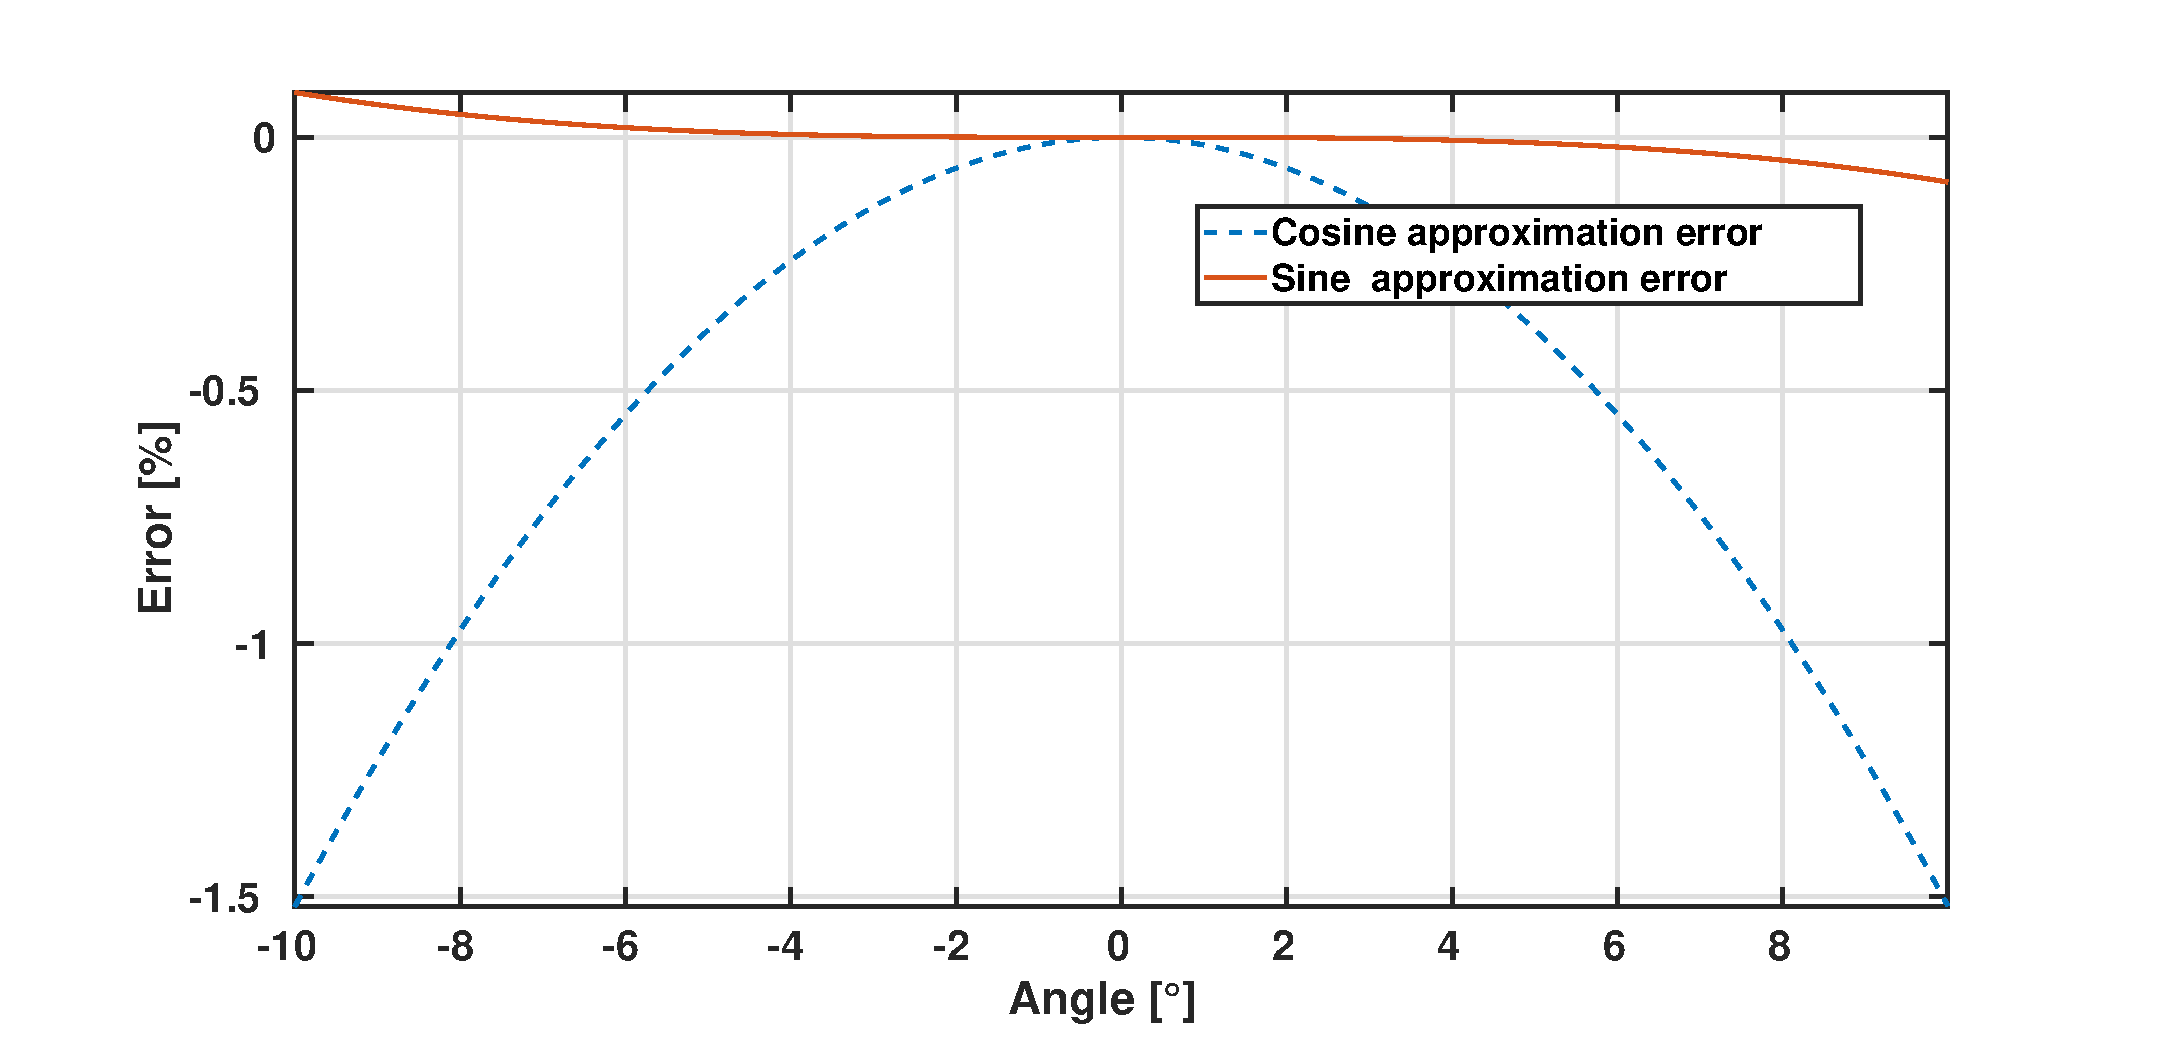
\includegraphics[width=0.8\textwidth]{CosSinLinApprox}
	\caption{Error generated by the approximation of the cosine and the sine function}\label{fig:BasLinPlot}
\end{figure}

